\documentclass[twocolumn]{jsarticle}
\usepackage[dvipdfmx]{graphicx}
\usepackage{sun}

\phiscalyear{2019}
\title{後醍醐天皇}
\author{Wikipedia}
\studentnumber{BS116000}

\begin{document}
\maketitle

\section{概要}

後醍醐天皇(ごだいごてんのう、1288年11月26日〈正応元年11月2日〉--1339年9月19日〈延元4年8月16日〉)は、日本の第96代天皇および南朝初代天皇(在位:1318年3月29日〈文保2年2月26日〉 - 1339年9月18日〈延元4年/暦応2年8月15日〉[注釈 2])。諱は尊治(たかはる)。

大覚寺統の天皇。元弘の乱で鎌倉幕府を倒して建武新政を実施したものの、間もなく足利尊氏との戦い建武の乱に敗れたため、大和吉野へ入り、南朝政権(吉野朝廷)を樹立し、尊氏の室町幕府が擁立した北朝との間で、南北朝の内乱を開始した。

主著に『建武年中行事』がある。

\begin{figure}[tbh]
\centering
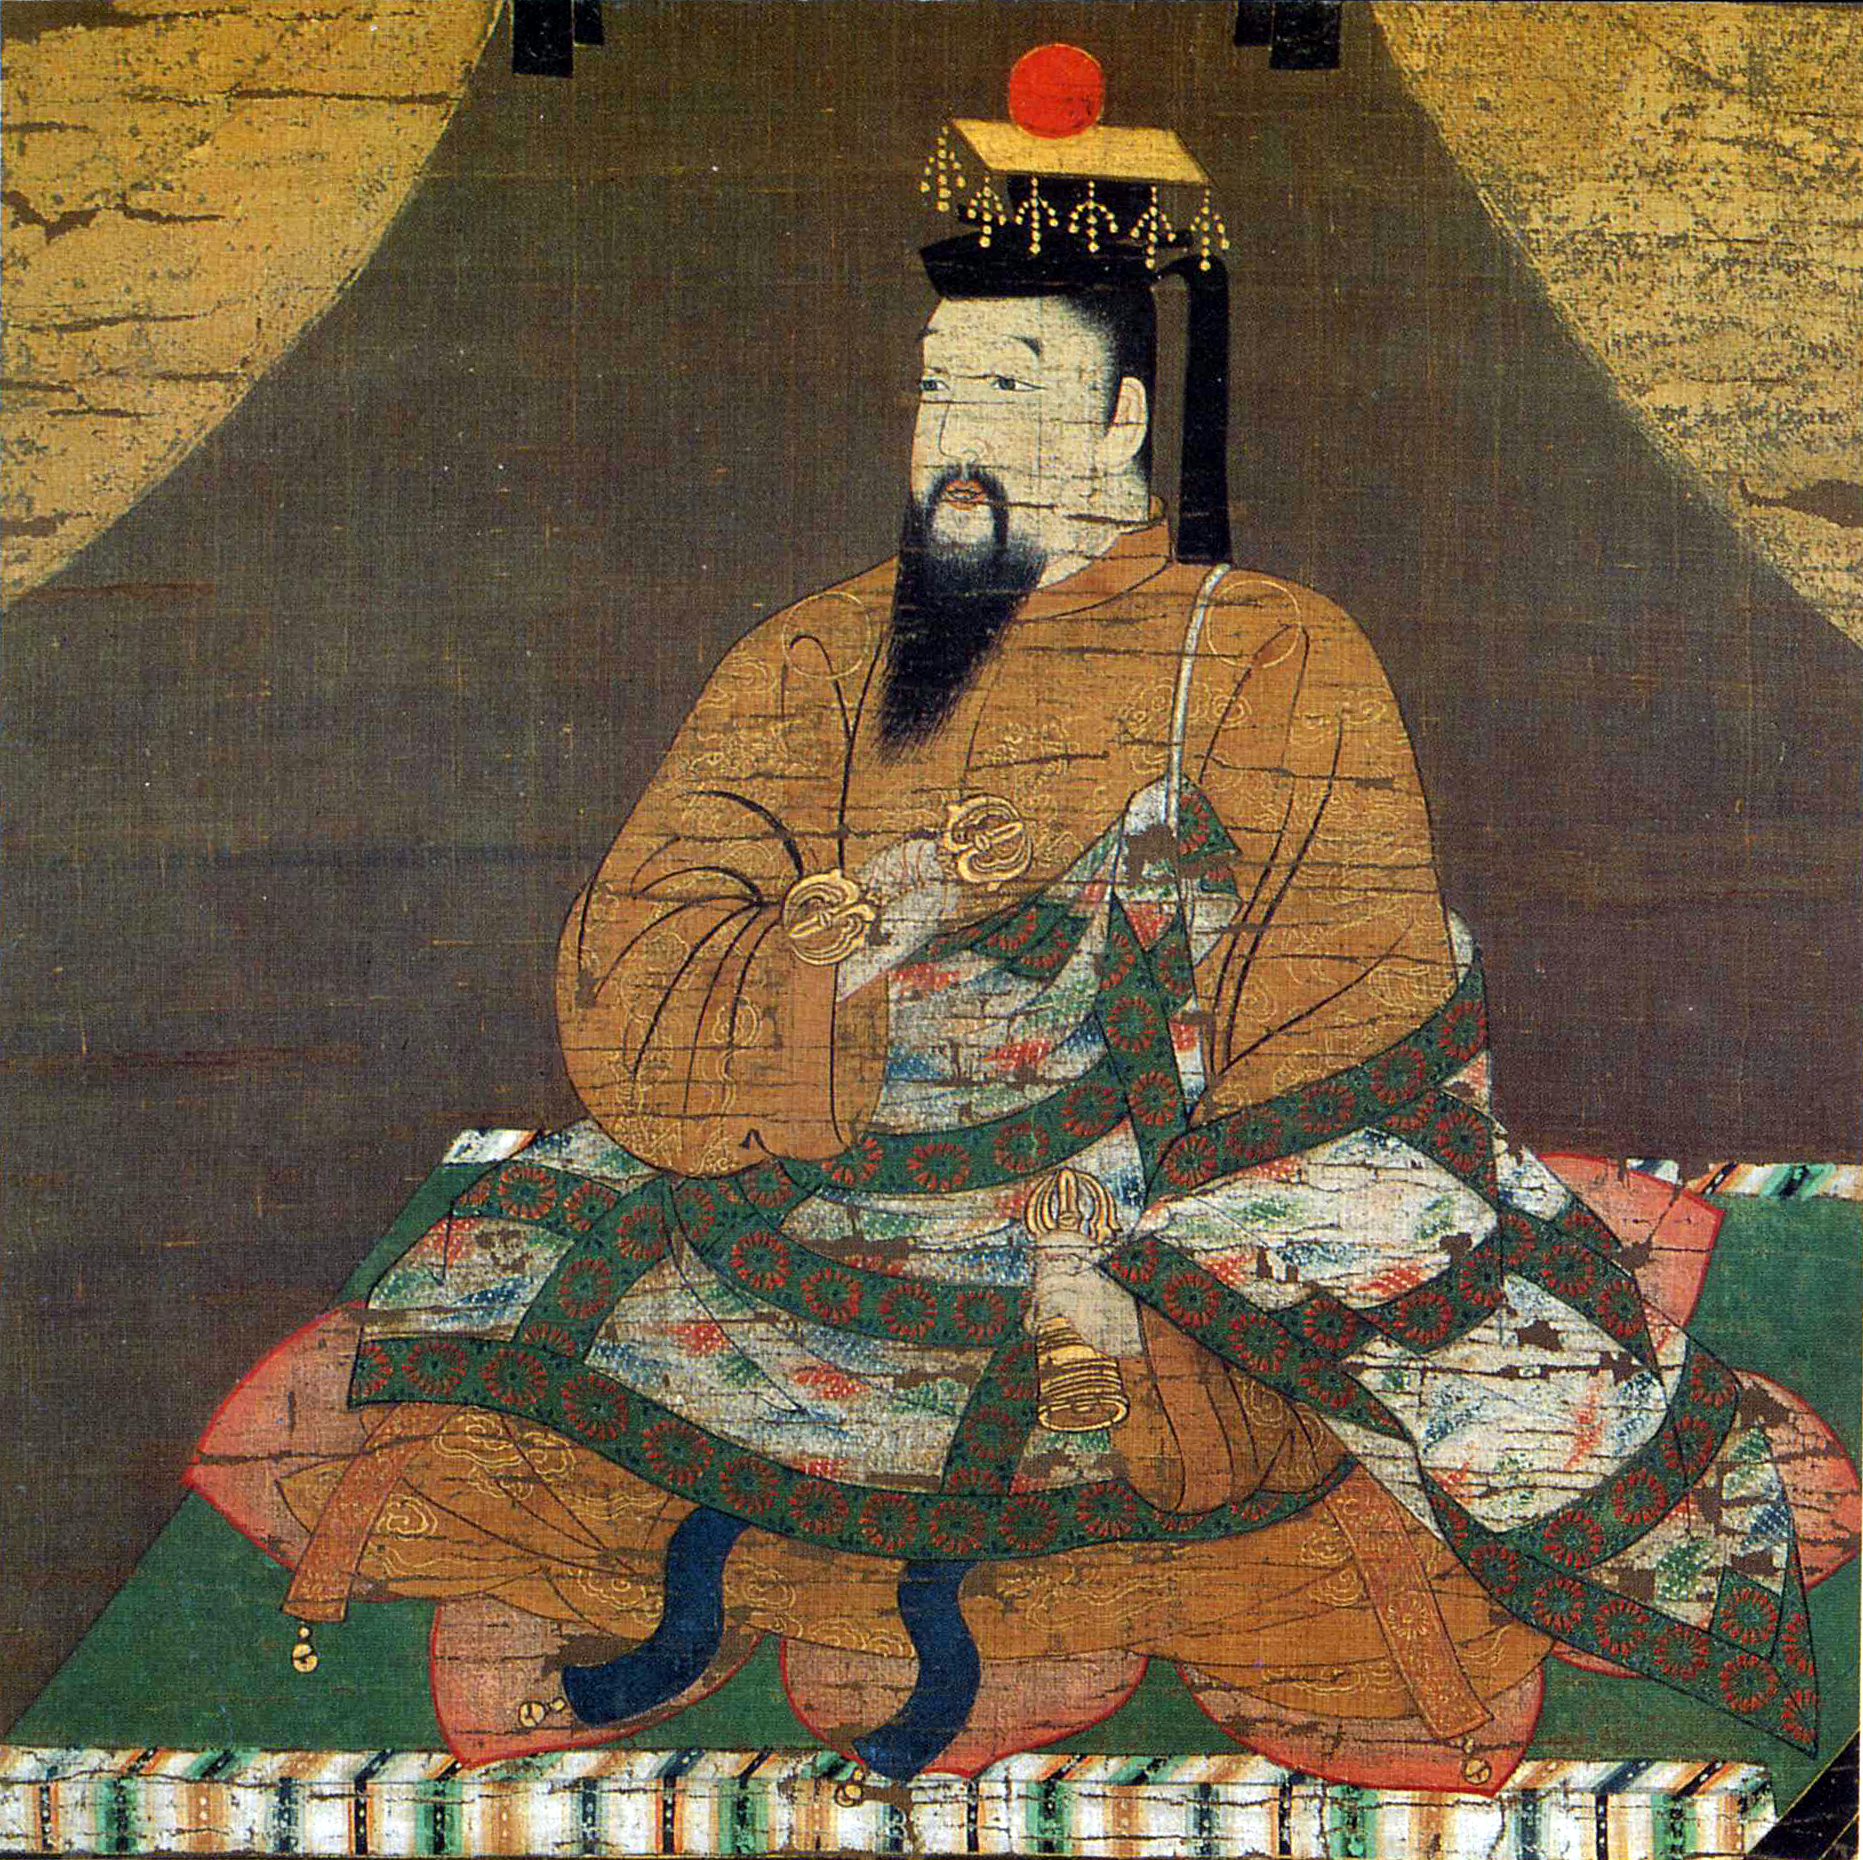
\includegraphics[keepaspectratio,scale=0.4]{Emperor_Godaigo.jpg}
\caption{文観開眼『後醍醐天皇像』(清浄光寺蔵、重要文化財)}
\label{fig:godaigo}
\end{figure}

\section{生涯}
\subsection{即位前}

大覚寺統・後宇多天皇の第二皇子。生母は、内大臣花山院師継の養女・藤原忠子(談天門院、実父は参議五辻忠継)。正応元年11月2日(1288年11月26日)に誕生し、正安4年(1302年)6月16日に親王宣下。嘉元元年(1303年)12月20日に三品に叙品。嘉元2年(1304年)3月7日に大宰帥となり、帥宮(そちのみや)と呼ばれた。また、徳治2年(1307年)5月15日には、中務卿を兼任している。

\subsection{即位}

徳治3年(1308年)に持明院統の花園天皇の即位に伴って皇太子に立てられ、文保2年2月26日(1318年3月29日)花園天皇の譲位を受けて31歳で践祚、3月29日(4月30日)に即位。30代での即位は1068年の後三条天皇の36歳での即位以来、250年ぶりであった。即位後3年間は父の後宇多法皇が院政を行った。後宇多法皇の遺言状に基づき、はじめから後醍醐天皇は兄後二条天皇の遺児である皇太子邦良親王が成人して皇位につくまでの中継ぎとして位置づけられていた。このため、自己の子孫に皇位を継がせることを否定された後醍醐天皇は不満を募らせ、後宇多法皇の皇位継承計画を承認し保障している鎌倉幕府への反感につながってゆく。元亨元年(1321年)、後宇多法皇は院政を停止して、後醍醐天皇の親政が開始される。前年に邦良親王に男子(康仁親王)が生まれて邦良親王への皇位継承の時機が熟したこの時期に後醍醐天皇が実質上の治天の君となったことは大きな謎とされる。

\subsection{倒幕計画}

正中元年(1324年)、後醍醐天皇の鎌倉幕府打倒計画が発覚して、六波羅探題が天皇側近日野資朝らを処分する正中の変が起こる。この変では、幕府は後醍醐天皇には何の処分もしなかった。天皇はその後も密かに倒幕を志し、醍醐寺の文観や法勝寺の円観などの僧を近習に近づけ、元徳2年(1329年)には中宮の御産祈祷と称して密かに関東調伏の祈祷を行い、興福寺や延暦寺など南都・叡山の寺社に赴いて寺社勢力と接近する(ただし、有力権門である西園寺家所生の親王は邦良親王系に対抗する有力な皇位継承者になり得るため、実際に御産祈祷が行われていた可能性もある)。大覚寺統に仕える貴族たちはもともと邦良親王を支持する者が大多数であり、持明院統や幕府も基本的に彼らを支持したため、後醍醐天皇は次第に窮地に陥ってゆく。そして邦良親王が病で薨去したあと、持明院統の嫡子量仁親王が幕府の指名で皇太子に立てられ、譲位の圧力はいっそう強まった。

\subsection{元弘の乱}

元弘元年(1331年)、再度の倒幕計画が側近吉田定房の密告により発覚し身辺に危険が迫ったため急遽京都脱出を決断、三種の神器を持って挙兵した。はじめ比叡山に拠ろうとして失敗し、笠置山(現京都府相楽郡笠置町内)に籠城するが、圧倒的な兵力を擁した幕府軍の前に落城して捕らえられる。これを元弘の乱(元弘の変)と呼ぶ。

幕府は後醍醐天皇が京都から逃亡するとただちに廃位し、皇太子量仁親王(光厳天皇)を即位させた。捕虜となった後醍醐は、承久の乱の先例に従って謀反人とされ、翌元弘2年 / 正慶元年(1332年)隠岐島に流された。この時期、後醍醐天皇の皇子護良親王や河内の楠木正成、播磨の赤松則村(円心)ら反幕勢力(悪党)が各地で活動していた。このような情勢の中、後醍醐は元弘3年 / 正慶2年(1333年)、名和長年ら名和一族を頼って隠岐島から脱出し、伯耆船上山(現鳥取県東伯郡琴浦町内)で挙兵する。これを追討するため幕府から派遣された足利高氏(尊氏)が後醍醐方に味方して六波羅探題を攻略。その直後に東国で挙兵した新田義貞は鎌倉を陥落させて北条氏を滅亡させる。

\subsection{建武の新政}

元弘3年6月5日(1333年7月17日)に帰京[1]した後醍醐天皇は、「今の例は昔の新義なり、朕が新儀は未来の先例たるべし」(『梅松論』上[2])と宣言し、建武の新政を開始した。なお、建武の新政については、当時から現在に至るまで多様な評価・解釈があり、その特徴や意義について一致した見解が得られていない。したがって、以下、本節では事象の列挙のみを行い、後醍醐天皇の政治思想やその意義・評価については「評価」の節に譲る。

まず、自らの退位と光厳天皇の即位を否定し、光厳朝で行われた人事をすべて無効にするとともに、幕府・摂関を廃した。両統迭立を廃止して皇統を大覚寺統に一統した。実子で元弘の乱に最初期から参戦した護良親王を征夷大将軍とし(数ヶ月後に解任)、足利高氏を戦功第一とし自身の諱(本名)「尊治」からの偏諱「尊氏」の名を与えて鎮守府将軍や参議などに任じた。同年中に記録所・恩賞方・雑訴決断所・武者所(頭人(長官)は新田義貞)・窪所などの重要機関が再興もしくは新設された。また、地方政権としては、親房の子北畠顕家を東北・北関東に(陸奥将軍府)、尊氏の弟足利直義を鎌倉に配置した(鎌倉将軍府)。

翌年(1334年)に入るとまず1月23日、父の後宇多天皇が大覚寺統嫡流に指定した甥の邦良親王の血統ではなく、実子の恒良親王を皇太子に立てた[3]。

同年1月29日(1334年3月5日)、簒奪者王莽を倒し後漢を開いた光武帝の元号の建武(けんぶ)の故事により、元号を建武(けんむ)に改元した[4]。

同年中に、検非違使庁による徳政令発布(5月3日)[5]、恩賞方の再編(5月18日)[6]、雑訴決断所の拡充(8月)[7]などの政策が行われた。また、硬貨・楮幣(紙幣)併用とする官銭乾坤通宝を計画し[8]、中御門宣明を鋳銭長官・五条頼元を鋳銭次官に任じた[9]。10月後半から11月初頭、護良親王が失脚し、足利直義に預けられ、鎌倉に蟄居となった(『梅松論』『保暦間記』『大乗院日記目録』)[10]。

建武2年(1335年)6月15日には造大内裏行事所始が行われた[11]。6月22日、大納言西園寺公宗の謀反が発覚し、武者所職員の楠木正成・高師直らに捕縛された[12]。

\subsection{足利尊氏との対立}

建武2年(1335年)、北条氏残党の北条時行が起こした中先代の乱の鎮圧のため勅許を得ないまま東国に出向いた足利尊氏が、乱の鎮圧に付き従った将士に鎌倉で独自に恩賞を与えた。これを新政からの離反と見なした後醍醐天皇は新田義貞に尊氏追討を命じ、義貞は箱根・竹ノ下の戦いでは敗れるものの、京都で楠木正成や北畠顕家らと連絡して足利軍を破った。尊氏は九州へ落ち延びるが、翌年に九州で態勢を立て直し、光厳上皇の院宣を得たのちに再び京都へ迫る。楠木正成は後醍醐天皇に尊氏との和睦を進言するが後醍醐天皇はこれを退け、義貞と正成に尊氏追討を命じた。しかし、新田・楠木軍は湊川の戦いで敗北し、正成は討死し義貞は都へ逃れた。

\subsection{南北朝時代}

足利軍が入京すると後醍醐天皇は比叡山に逃れて抵抗するが、足利方の和睦の要請に応じて三種の神器を足利方へ渡し、尊氏は光厳上皇の院政のもとで持明院統から光明天皇を新天皇に擁立し、建武式目を制定して幕府を開設する(なお、太平記の伝えるところでは、後醍醐天皇は比叡山から下山するに際し、先手を打って恒良親王に譲位したとされる)。廃帝後醍醐は幽閉されていた花山院を脱出し、尊氏に渡した神器は贋物であるとして、吉野(現奈良県吉野郡吉野町)に自ら主宰する朝廷を開き、京都朝廷(北朝)と吉野朝廷(南朝)が並立する南北朝時代が始まる。後醍醐天皇は、尊良親王や恒良親王らを新田義貞に奉じさせて北陸へ向かわせ、懐良親王を征西将軍に任じて九州へ、宗良親王を東国へ、義良親王を奥州へと、各地に自分の皇子を送って北朝方に対抗させようとした。しかし、劣勢を覆すことができないまま病に倒れ、延元4年 / 暦応2年(1339年)8月15日、奥州に至らず、吉野へ戻っていた義良親王(後村上天皇)に譲位し、翌日、吉野金輪王寺で朝敵討滅・京都奪回を遺言して崩御した。享年52(満50歳没)。

摂津国の住吉行宮にあった後村上天皇は、南朝方の住吉大社の宮司である津守氏の荘厳浄土寺において後醍醐天皇の大法要を行う。また、尊氏は後醍醐天皇を弔い、京都に天竜寺を造営している。


\end{document}